% タイトル
\chapter{角の三等分問題}
\vspace{-45pt} %高さ調整
\begin{flushright}
  {\bf \large 理工学部 物理科学科 2回生} \\ \vspace{3pt} %所属
  {\bf \large 中山 敦貴} \\ \vspace{30pt} %名前
\end{flushright}

% 序論
\section*{はじめに}
高2のころから読み始めた結城浩さん著の「数学ガール」であるが、今年の夏休みにようやく第5巻であるガロア理論を読み終えることができた。よって今回の内容はガロア理論である。と言いたいところだが、ガロア理論なんて簡単に理解できるものじゃないし、代数学のラスボスである(適当)。ということで今回は代数学超入門として、作図可能数の話をすることにする。また、他にも2冊ガロア理論超入門書を読んで、方程式の面白い話があったのでそれも紹介したかったが、今回の会誌には入れることができなかった。今後作るかもしれないバージョンアップ版に期待してほしい。

%
\section{角の三等分問題とは}
有名な作図問題のひとつに、角の三等分問題というものがある。今回はこれ考えるわけであるが、まずは数学的にどのような問いになっているか考えよう。
\begin{itembox}[l]{\bf 角の三等分問題(?)}
{\bf 問い} 与えられた角を三等分できるか?\\
{\bf 解答} 分度器使えばできる。
\end{itembox}
\par 問いたいことはそういうことじゃない。もう少しちゃんと問いを立てよう。\\

\begin{itembox}[l]{\bf 角の三等分問題}
{\gt 定規}と{\gt コンパス}だけを使って、与えられた{\gt 任意の}角を三等分できるか?
\end{itembox}

\begin{quote}
{\gt 定規}  :与えられた2点を通る直線が引ける。\\
{\gt コンバス}:与えられた2点の片方を中心とし、他方を通る円が描ける。
\end{quote}

\begin{itemize}
\item[{\gt (注)}]
\item 初めに2点は与えられているとする。
\item 定規とコンパスは繰り返し使える(ただし有限回とする)。
\item ある時点で使える点は、そこまでに作図した「直線と円」「直線と直線」「円と円」の交点だけとする。
\item コンパスで円を書いた後、コンパスの針を他の点に移して円を描いてもよいとする(=同じ半径の円を別の点の周りに描いてもよい)。
\end{itemize}

つまり、三等分できないような角が1つでもあれば、”定規とコンパスだけでは、与えられた任意の角を三等分{\gt できない}”というのがこの角三等分問題への解答となる。オチを言ってしまうと、実際そうなっている。つまり定規とコンパスだけで三等分できないような角が存在する。それも身近なところに。

%
\section{作図可能数}

\subsection{作図可能数とは}
作図には{\gt 点}が必要だから、{\gt 作図可能な点}$(x,y)$を考えることになる。作図可能点の座標成分$x,y$を{\gt 作図可能数}と呼ぶ。\par
では、いったいどんな数が作図可能数になっているだろうか?\par
まず初めに、原点$(0,0)$と$(1,0)$の2点が与えられているとする。
原点$(0,0)$と$(1,0)$を通る直線を引けば$x$軸ができる。さらにコンパスを使って、$x$軸上に整数の点を作図できる。$x$軸に対して原点を通るように垂線を引けば$y$軸もでき、$y$軸上にも整数の点が作図できる。つまり格子点が作図できることになる。よって、{\gt 整数は作図可能数}となる。

\newpage
\subsection{四則演算と開平}
以下のようにすれば、定規とコンパスで加減乗除ができる。
\begin{figure}[H]
  \begin{center}
    \begin{tabular}{c}
        \begin{minipage}{0.5\hsize}
          \begin{center}
            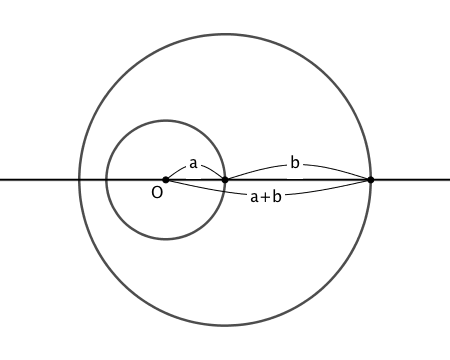
\includegraphics[clip, width=5.5cm]{nakayama2/image/a+b.png}
            \hspace{1.6cm} \bf $a$と$b$から$a+b$をつくるの図
          \end{center}
        \end{minipage}

        \begin{minipage}{0.5\hsize}
          \begin{center}
            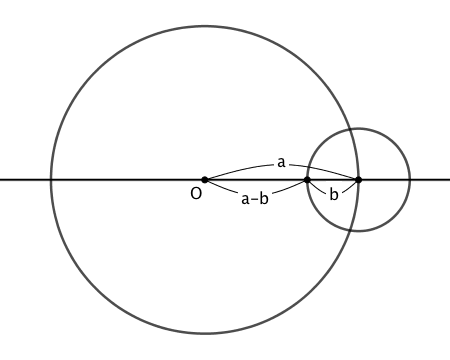
\includegraphics[clip, width=5.5cm]{nakayama2/image/a-b.png}
            \hspace{1.6cm} \bf $a$と$b$から$a-b$をつくるの図
          \end{center}
        \end{minipage}
    \end{tabular}
  \end{center}
\end{figure}\par

\begin{figure}[H]
  \begin{center}
    \begin{tabular}{c}
        \begin{minipage}{0.5\hsize}
          \begin{center}
            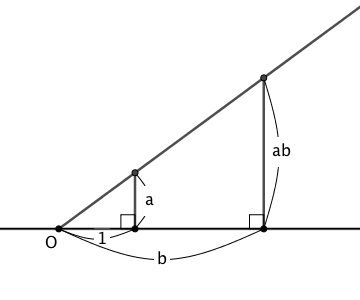
\includegraphics[clip, width=5.5cm]{nakayama2/image/ab.png}
            \hspace{1.6cm} \bf $a$と$b$から$ab$をつくるの図
          \end{center}
        \end{minipage}

        \begin{minipage}{0.5\hsize}
          \begin{center}
            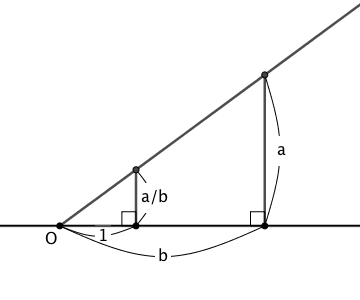
\includegraphics[clip, width=5.5cm]{nakayama2/image/a_b.png}
            \hspace{1.6cm} \bf $a$と$b$から$\frac{a}{b}$をつくるの図
          \end{center}
        \end{minipage}
    \end{tabular}
  \end{center}
\end{figure}\par\par\par

整数が作図可能で加減乗除ができるので、整数の加減乗除で作られる{\gt 有理数は作図可能数}となる。
作図で加減乗除ができるので、作図可能数は{\gt 体}$(\DD とする)$である。
$$\mathbb{Z} \subset \mathbb{Q} \subset \DD \subset \mathbb{R}$$
さらに、定規とコンパスで開平もできる。下図で、三平方の定理より、$\mathrm{BP} = \sqrt{a}$となっていることがわかる。

\begin{figure}[H]
  \centering
  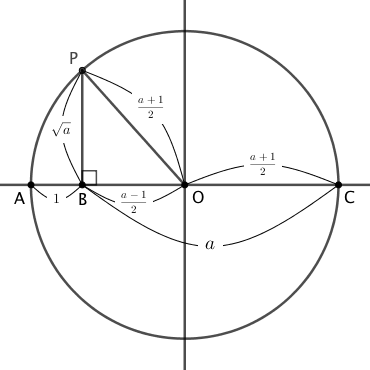
\includegraphics[clip, width=7cm]{nakayama2/image/root.png}\\
  \bf $a$から$\sqrt{a}$をつくるの図
\end{figure}

よって
\begin{align*}
  \sqrt{a} \in \DD \qquad (a \in \mathbb{Q},\, a > 0)
\end{align*}
さらに開平を繰り返してもよい
\begin{align*}
  a \in \DD \Rightarrow \sqrt{a} \in \DD \qquad (a > 0)
\end{align*}
つまり、$a$を正の有理数として次のようなことがいえる:
\begin{align*}
  \sqrt{a} \in \DD\\
  \sqrt{\sqrt{a}} \in \DD\\
  \sqrt{\sqrt{\sqrt{a}}} \in \DD\\
\end{align*}
さらにそうして作った数の加減乗除もできるので、$p,q,r$を正の有理数として次のようなこともいえる:
\begin{align*}
  \sqrt{\sqrt{p} + \sqrt{q}} \in \DD\\
  \sqrt{\sqrt{p} + \sqrt{\sqrt{q}}} + \sqrt{r} \in \DD\\
  \sqrt{\sqrt{\sqrt{p} + \sqrt{\sqrt{q}}} + \sqrt{r}} \in \DD\\
\end{align*}\par
整数から始めて加減乗除と開平を繰り返し使えばどんな数でも作れそうだが、そんなことはない。例えば$\sqrt[3]{2}$は整数の加減乗除と開平だけからは作れない。
\begin{quote}
  じゃあ結局どんな数が作図できるの?
\end{quote}
直線は1次方程式、円は2次方程式で書ける。その交点(作図可能点)は連立方程式で求められる。連立方程式には1次方程式と2次方程式しか出てこないので、作図可能数は1次方程式か2次方程式の解になるものしかない。
よって作図可能数は
\begin{quote}
  《加減乗除と開平の繰り返しで作れる数》
\end{quote}
であることがわかる。

%
\section{本題}
\subsection{$20^\circ$の作図}
それでは、作図可能数を用いて角の三等分問題を考える。\par
$20^\circ$が作図可能かどうか調べよう。もし$20^\circ$が作図可能でなければ、それが角三等分問題への解答となる。
$$
20^\circ\text{が作図可能} \,\,\Longleftrightarrow\,\, \cos 20^\circ \text{が作図可能数}
$$
であるから$\cos 20^\circ$が作図可能数か考えればよい。
\begin{figure}[H]
  \centering
  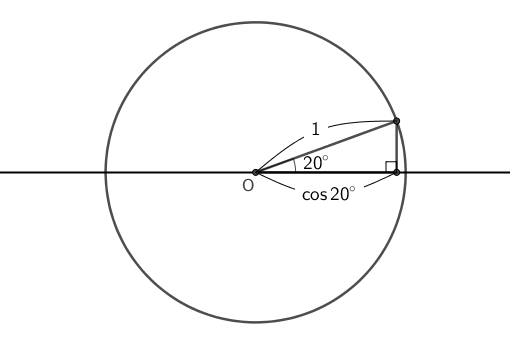
\includegraphics[clip, width=5.5cm]{nakayama2/image/cos20do.png}\\
  \small $20^\circ$が作図できれば$\cos 20^\circ$も作図可能。逆も言える。
\end{figure}

コサインの三倍角公式「$\cos 3\theta = 4\cos^3 \theta - 3\cos\theta$」で$\theta = 20^\circ$としてみると
\begin{align*}
  \cos 60^\circ = 4\cos^3 20^\circ - 3\cos 20^\circ \\
  \frac{1}{2} = 4\cos^3 20^\circ - 3\cos 20^\circ \\
  8\cos^3 20^\circ - 6\cos 20^\circ - 1 = 0
\end{align*}
$x = 2\cos 20^\circ$とおくと
$$ x^3 - 3x -1 = 0 $$
となり、この3次方程式の解の1つが$2\cos 20^\circ$になっている。
よって、もしこの3次方程式が作図可能数を1つも解に持たないならば、$2\cos 20^\circ$つまり$\cos 20^\circ$は作図可能数でないことになる。
したがって$20^\circ$は作図不可能となり、三等分できない角として$60^\circ$が与えられる。


\subsection{証明!証明!証明!}
\subsubsection{証明の概要}
もうただ真面目に証明してしまうことにする。
\begin{itembox}[l]{\bf 定義}
  $0$以上の整数$n$について、体$\KK_n$を以下のように定義する:
  \begin{align*}
    \begin{cases}
    \,\KK_0 &= \mathbb{Q}\\
    \,\KK_{k+1} &= \{p + q\sqrt{r} \,\,|\,\, p,q,r \in \KK_k, \sqrt{r} \notin \KK_k\}\\
    & \qquad\text{\footnotesize (ただし$k = 0,1,2,...$で$r$は$k$ごとに固定する)}\\
    &= \KK_k (\sqrt{r}) \qquad\text{$r \in \KK_k, \sqrt{r} \notin \KK_k$}
    \end{cases}
  \end{align*}
\end{itembox}
\,
\begin{itembox}[l]{\bf 定義}
  命題$P(n)$:方程式$x^3 -3x -1 = 0$は、体$\KK_n$に解を持たない
\end{itembox}
\,
\begin{itembox}[l]{\bf 証明すべきこと}
  以下のステップ(a)とステップ(b)を示せば、数学的帰納法により、どんな$0$以上の整数$n$についても$P(n)$が成り立つ。すなわち、方程式$x^3 -3x -1 = 0$は、体$\KK_n$に解を持たない。
  \begin{quote}
    ステップ(a):$P(0)$\\
    ステップ(b):$P(k) \Rightarrow P(k+1)$
  \end{quote}
\end{itembox}

% \clearpage
\subsubsection{ステップ(a)}
\begin{itembox}[l]{\bf ステップ(a)}
  方程式$x^3 -3x -1 = 0$は有理数体$\mathbb{Q}$に解を持たない
\end{itembox}
{\bf (証明)}\par
方程式$x^3 -3x -1 = 0$は有理数体$\mathbb{Q}$に解を持つと仮定する。\par
すると解$x$は整数$A,B$を用いて次のように表せる:
$$ x = \frac{A}{B} \qquad (B \neq 0,\, AとBは互いに素)$$\par
これを$x^3 -3x -1 = 0$に代入して整理すると
$$ A^3 = (3A + B)B^2 $$\par
ここで$A$の素因数に注目する。まず$A \neq 0,1,-1$であることは、それぞれ代入してみればわかる。また、$A < 0$のときは$B$の符号を反転させればよいので、$A > 0$の場合だけ考える。\par
$A$の素因数を$p$とすると、左辺$A^3$は$p$で割り切れる。しかし右辺の$(3A+B)$も$B^2$も$p$で割り切れない。$\rightarrow$矛盾
\begin{flushright}
  (証明終)
\end{flushright}

\subsubsection{ステップ(b)}

あとで使うので、まず補題を1つ証明しておく。$\KK = \mathbb{Q}$のときはもう中学生か高校生のころに証明したことがあると思う。それの一般化である。
\begin{itembox}[l]{\bf 補題}
$\KK$を体とし、$p,q,r \in \KK, \sqrt{r} \notin \KK$のとき
$$ p + q\sqrt{r} = 0 \,\,\Longleftrightarrow\,\, p = q = 0$$
\end{itembox}
{\bf (証明)}\\
$(\Leftarrow)$であること \par $p = q = 0$なら明らかに$p + q\sqrt{r} = 0$ \\
$(\Rightarrow)$であること \par
仮定より$p + q\sqrt{r} = 0$。 \par
$q = 0$ならば$p = 0$。\par
$q \neq 0$のとき、$\sqrt{r} = -\frac{p}{q}$。\par
ここで$\sqrt{r} \notin \KK$ であるが、$-\frac{p}{q} \in \KK$となっている。 $\rightarrow$矛盾\par
よって$q = 0$。
\begin{flushright}
  (証明終)
\end{flushright}


\begin{itembox}[l]{\bf ステップ(b)}
方程式$x^3 -3x -1 = 0$は体$\KK$に解を持たない $\Longrightarrow$ 体$\KK(\sqrt{r})$にも解を持たない
\end{itembox}
{\bf (証明)}\par
前提条件:方程式$x^3 -3x -1 = 0$は体$\KK$に解を持たない\par
仮定:方程式$x^3 -3x -1 = 0$は体$\KK(\sqrt{r})$に解を持つ\par
その解を$x = p + q\sqrt{r} \in \KK(\sqrt{r})$とする。$(p,q,r \in \KK, \sqrt{r} \notin \KK)$\par
ここで$q \neq 0, r \neq 0$である。(\,$\because$ 前提条件に反する)\par
$x^3 -3x -1 = 0$に$x = p + q\sqrt{r}$を代入して整理すると
$$ (p^3 - 3p - 1 + 3pq^2r) + (3p^2 + q^2r - 3)q\sqrt{r} = 0 $$
となる。ここで$P = (p^3 - 3p - 1 + 3pq^2r), Q = (3p^2 + q^2r - 3)q$とおけば、$P,Q \in \KK$であり、
$$ P + Q\sqrt{r} = 0 $$
と書ける。\par
また、$x^3 -3x -1$に$x = p - q\sqrt{r}$を代入してみると
\begin{align*}
  x^3 -3x -1 &= (p^3 - 3p - 1 + 3pq^2r) - (3p^2 + q^2r - 3)q\sqrt{r}\\
  &= P - Q\sqrt{r}
\end{align*}
となる。\par
ここで補題より$P = Q = 0$であり、$P - Q\sqrt{r} = 0$となる。すなわち$p + q\sqrt{r}$が解のとき、$p - q\sqrt{r}$も解となっている。\par
3次方程式は3つの解を持つが、そのうちの2つは既に分かっている。
\begin{align*}
  \begin{cases}
    \,\alpha &= p + q\sqrt{r}\\
    \,\beta &= p - q\sqrt{r}\\
    \,\gamma &= \,\,\,?
  \end{cases}
\end{align*}\par
3つ目の解$\gamma$は解と係数の関係$\alpha + \beta + \gamma = 0$より
\begin{align*}
  \gamma &= - \alpha - \beta \\
  &= -(p + q\sqrt{r}) - (p - q\sqrt{r})\\
  &= -2p
\end{align*}\par
ここで$p \in \KK$より$\gamma = -2p \in \KK$となるが、これは前提条件に反する。\par
よって仮定が否定され、
\begin{quote}
  《方程式$x^3 -3x -1 = 0$は体$\KK$に解を持たない》という前提条件で\\
  《方程式$x^3 -3x -1 = 0$は体$\KK(\sqrt{r})$に解を持たない》
\end{quote}
ということが証明できた。
\begin{flushright}
  (証明終)
\end{flushright}

\subsection{拡大次数を用いた別の証明}
体の話をいろいろと知っているともっとスマートに証明ができる。これからその証明を紹介するが、僕も体の話はよく知らない。なのでいくつかの定理というか拡大次数を求めるための公式を証明はせずに、具体例をいくつか見てもらうことでその定理が正しいと納得してもらうことにする。
\begin{itembox}[l]{\bf 拡大体$\mathbb{Q}(a)/\mathbb{Q}$}
$\mathbb{Q}$:有理数体\par
$\mathbb{Q}(a)$:有理数体$\mathbb{Q}$に数$a$を添加した体\par
としたとき、
$\mathbb{Q}(a)$は$\mathbb{Q}$の{\gt 拡大体}であることを$\mathbb{Q}(a)/\mathbb{Q}$と書く。
\end{itembox}

\begin{itembox}[l]{\bf $\mathbb{Q}(a)/\mathbb{Q}$の拡大次数}
$\mathbb{Q}(a)$を$\mathbb{Q}$上の線形空間とみなしたときの{\gt 次元}(基底の要素数)を$\mathbb{Q}(a)/\mathbb{Q}$の{\gt 拡大次数}といい、$[\mathbb{Q}(a):\mathbb{Q}]$と書く。\\
拡大次数が$n$になる体の拡大を{\gt $n$次拡大}という。
\end{itembox}
{\gt 例}\par
$\mathbb{Q}(\sqrt{2}) = \{p + q\sqrt{2} \,\,|\,\, p,q \in \mathbb{Q}\}$ \par
$\mathbb{Q}(\sqrt{2})$に属する任意の数は$\{ 1, \sqrt{2} \}$という2つの基底を使って$p + q\sqrt{2}$と書ける。\par
よって、$\mathbb{Q}(\sqrt{2})/\mathbb{Q}$の拡大次数は
$$[\mathbb{Q}(a):\mathbb{Q}] = 2$$
となり、この拡大は2次拡大である。

\begin{itembox}[l]{\bf 拡大次数の積の定理}
$\mathbb{Q}$に数$a,b$を添加した拡大体
$$\mathbb{Q}(a,b) = \mathbb{Q}(a)(b) \quad \text{($\mathbb{Q}(a)$に$b$を添加した体)}$$
の拡大次数は
\begin{align*}
  [\mathbb{Q}(a,b):\mathbb{Q}] &= [\mathbb{Q}(a)(b):\mathbb{Q}]\\
  &= [\mathbb{Q}(a):\mathbb{Q}] \times [\mathbb{Q}(a)(b):\mathbb{Q}(a)]
\end{align*}
で計算できる。
\end{itembox}
{\gt 例1}
\begin{align*}
  [\mathbb{Q}(\sqrt{2},\sqrt{3}):\mathbb{Q}] &= [\mathbb{Q}(\sqrt{2})(\sqrt{3}):\mathbb{Q}]\\
  &= [\mathbb{Q}(\sqrt{2}):\mathbb{Q}] \times [\mathbb{Q}(\sqrt{2})(\sqrt{3}):\mathbb{Q}(\sqrt{2})]\\
  &= 2 \times 2 = 4
\end{align*}\par
実際、基底は$\{ 1,\sqrt{2},\sqrt{3},\sqrt{6} \}$の4つ。\\\\
{\gt 例2}
\begin{align*}
  [\mathbb{Q}(\sqrt{2},\sqrt{3},\sqrt{5},\sqrt{7}):\mathbb{Q}] &= [\mathbb{Q}(\sqrt{2})(\sqrt{3})(\sqrt{5})(\sqrt{7}):\mathbb{Q}]\\
  &= [\mathbb{Q}(\sqrt{2}):\mathbb{Q}] \\
  &\qquad \times [\mathbb{Q}(\sqrt{2})(\sqrt{3}):\mathbb{Q}(\sqrt{2})]\\
  &\qquad\qquad \times [\mathbb{Q}(\sqrt{2})(\sqrt{3})(\sqrt{5}):\mathbb{Q}(\sqrt{2})(\sqrt{3})] \\
  &\qquad\qquad\qquad \times  [\mathbb{Q}(\sqrt{2})(\sqrt{3})(\sqrt{5})(\sqrt{7}):\mathbb{Q}(\sqrt{2})(\sqrt{3})(\sqrt{5})] \\
  &= 2 \times 2 \times 2 \times 2  \\
  &= 16
\end{align*}

\begin{itembox}[l]{\bf 定理}
複素数$\theta$に対し、以下の条件を満たす有理数係数の$n$次多項式$p(x)$が存在するとき、多項式$p(x)$を、数$\theta$の$\mathbb{Q}$上の最小多項式という。
\begin{itemize}
\item $p(x)$は$\theta$を根に持つ。
\item $p(x)$の$n$次の係数は$1$に等しい。
\item $\theta$を根に持つ、$n$次未満の有理数係数の多項式は存在しない。
\end{itemize}
またこのとき、体の拡大$\mathbb{Q}(\theta)/\mathbb{Q}$を$\mathbb{Q}$上の線形空間と考えると、
$$ \{ 1, \theta, \theta^2, \theta^3, \cdots, \theta^{n-1} \} $$
は基底となる。
\end{itembox}
\newpage
{\gt 例}\par
$\sqrt{2} + \sqrt{3}$の最小多項式は
\begin{align*}
  x &= \sqrt{2} + \sqrt{3}\\
  x^2 &= (\sqrt{2} + \sqrt{3})^2\\
  x^2 &= 5 + 2\sqrt{6}\\
  x^2 - 5 &= 2\sqrt{6}\\
  (x^2 - 5)^2 &= (2\sqrt{6})^2\\
  x^4 - 10x^2 + 1 &= 0
\end{align*}
と4次方程式になるので、拡大体$\mathbb{Q}(\sqrt{2} + \sqrt{3})$を$\mathbb{Q}$上の線形空間とみなしたとき
$$ \{ 1, \sqrt{2} + \sqrt{3}, (\sqrt{2} + \sqrt{3})^2, (\sqrt{2} + \sqrt{3})^3 \} $$
は基底となる。また、拡大次数は
$$[\mathbb{Q}(\sqrt{2} + \sqrt{3}):\mathbb{Q}] = 4$$
とわかる。

\subsubsection{拡大次数を用いた"簡潔な"証明}
作図可能数とは、$0$と$1$から始めて、加減乗除と開平を有限回使って作られる数のこと。つまり作図可能数体は、有理数体$\mathbb{Q}$に2次拡大($\sqrt{~~}$を添加)を有限回繰り返して作られる体となる。よって、$\alpha$を作図可能数としたとき、$\mathbb{Q}(\alpha)/\mathbb{Q}$の拡大次数は$2^n$に等しい。
$$ [\mathbb{Q}(\alpha):\mathbb{Q}] = 2^n \quad(\alpha:作図可能数) $$
一方、$2\cos 20^\circ$の$\mathbb{Q}$上の最小多項式が$x^3 - 3x - 1$であることから、$\cos 20^\circ$の$\mathbb{Q}$上の最小多項式が$x^3 - \frac{3}{4}x - \frac{1}{8}$であることがわかる。したがって$\mathbb{Q}(\cos 20^\circ)/\mathbb{Q}$の拡大次数は3となる。
$$ [\mathbb{Q}(\cos 20^\circ):\mathbb{Q}] = 3 $$
しかし$2^n = 3$を満たす整数$n \ge 0$は存在しないので、$\cos 20^\circ$は作図可能数でない。よって定規とコンパスで$20^\circ$は作図不可能。つまり、定規とコンパスで$60^\circ$を三等分することは不可能である。\par
これで角の三等分問題が証明できた。

%
\clearpage
\section{おまけ}
時間の都合で実際に計算することはできなかったが、正17角形が作図可能かどうかは、$\cos \frac{2\pi}{17}$が作図可能数であるかどうか調べればよい。結果は以下のように(四則演算と開平だけで)かけるので、正17角形は作図可能である。
\begin{screen}
  正17角形が作図可能であることを表す式
  \begin{align*}
    \cos \frac{2\pi}{17} &= -\frac{1}{16} + \frac{1}{16}\sqrt{17} + \frac{1}{16}\sqrt{2(17 - \sqrt{17})}\\
    & \hspace{8mm} + \frac{2}{16}\sqrt{17 + 3\sqrt{17} - \sqrt{2(17 - \sqrt{17})} - 2\sqrt{2(17 - \sqrt{17})}}
  \end{align*}
\end{screen}\par
ちなみに$\cos \frac{2\pi}{17}$は17次方程式
$$ x^{17} = 1$$
の非自明な解の1つであるから、これを代数的に解けば上の式が正しいことがわかる。\par
ぜひ考えてほしい。(この辺が今回は入りきらなかった内容。)

%
\section*{参考文献}
\begin{enumerate}
  \item 結城浩、『数学ガール/ガロア理論』、ソフトバンククリエイティブ、2012年。
\end{enumerate}

%
